\section{Proof for rank 5}


\subsection{Basic results}

\paragraph{}
Dans la suite, nous noterons les carrés alternés grâce au deux involutions qui les composent. Un carré alterné avec des arêtes $\rho_0$ et $\rho_2$ sera noté $[\rho_0, \rho_2]$.

\begin{definition}
  Deux carrés alternés sont dit adjacents s'ils partagent deux sommets\footnote{Ces définitions sont à améliorer, il y a quelques problèmes mais je pense qu'il y a moyen de rendre ça correct}.
\end{definition}

\begin{definition}
  Une suite de carrés alternés adjacents est un suite finie dans laquelle chaque carré alterné est adjacent avec son précédesseur et son successeur s'ils existent.
\end{definition}

\begin{definition}
  Une suite de carré alternés adjacents est dite linéaire si une des deux composante de sa notation est constante.
\end{definition}

Par exemple, la suite $[\rho_0, \rho_2], [\rho_0, \rho_4], [\rho_0, \rho_3]$ est linéaire car la première composante est toujours $\rho_0$.

\begin{definition}
  Une suite de carré alterné est dite monotone si la suite formée par les différences des indices de ses carrés est monotone.
\end{definition}

La suite $[\rho_0, \rho_2], [\rho_0, \rho_3], [\rho_0, \rho_4]$ est monotone, en effet la suite formée par la différente des indice est $2, 3, 4$ et cette suite est bien monotone.

\begin{proposition}
  Toute suite de carrés alternés monotone est linéaire.
\end{proposition}

\begin{proof}
  Une suite monotone non-linéaire serait de la forme suivante: $[\rho_{i-1}, \rho_j], [\rho_i, \rho_j], [\rho_i, \rho_{j+1}]$, si nous représentons le graphe d'une telle suite nous obtenons le graphe suivant:

  \begin{figure}[H]
    \begin{center}
      \begin{tikzpicture}

        \begin{scope}[every node/.style={circle,draw}]
          \node (1)  at (0,2)  {};
          \node (2)  at (0,0)  {};
          \node (3)  at (0,-2) {};
          \node (4)  at (2,2)  {};
          \node (5)  at (2,0)  {};
          \node (6)  at (2,-2) {};
          \node (7)  at (4,2)  {};
          \node (8)  at (4,0)  {};
        \end{scope}

        \begin{scope}[every node/.style={fill=white,circle}]

          \begin{scope}[every edge/.style={draw}]
            \path (2)  edge node {$i-1$} (3);
            \path (5)  edge node {$i-1$} (6);
            \path (1)  edge node {$i$} (2);
            \path (4)  edge node {$i$} (5);
            \path (7)  edge node {$i$} (8);
            \path (1)  edge node {$j$} (4);
            \path (2)  edge node {$j$} (5);
            \path (3)  edge node {$j$} (6);
            \path (4)  edge node {$j+1$} (7);
            \path (5)  edge node {$j+1$} (8);
          \end{scope}
        \end{scope}

      \end{tikzpicture}
      \caption{Suite de carrés alternés monotone et non-linéaire}
    \end{center}
  \end{figure}

  \paragraph{}
  Nous avons un problème en bas à droite, nous ne pouvons pas ajouter de carré à cet endroit sinon nous n'avons plus une suite, donc il faut que $i-1$ et $j+1$ soit consécutifs. On a alors $i = j+1$ ou $i+1=j$ étant donné la symétrie nous pouvons n'en conserver qu'une. Prenons $i = j+1$, ceci est un problème car alors notre carré alterné $[\rho_i, \rho_j]$ n'en est plus un, en effet $|i-j| = 1$.

\end{proof}

\begin{lemma}
  La parité de la taille d'une suite de carrés alternés est toujours la même que la partité d'une suite monotone qui admet les deux même extrémités.
\end{lemma}

\begin{lemma}
  Si on a un carré alterné dont les indices différent de plus 2 alors le seul moyen de l'étendre est d'utiliser un autre carré alterné.
\end{lemma}

\begin{corollary}
  Si nous travaillons sur un nombre impair de points et si nous avons un carré alterné dont la différence des indices est de plus de 2, alors toute extension de ce carré alterné à tous les points contient une suite de carrés alternés qui comprend un carré dont la différence des indices est exactement 2.
\end{corollary}

\begin{proof}
  Chaque fois que nous étendons avec un carré alterné nous ajoutons deux points. Si nous avons un nombre impair de points alors nous ne pouvons pas utiliser que des carrés alternés pour les relier. Mais si nous avons un carré alterné dont la différence des indices est de plus de deux, nous devons forcément l'étendre à un autre carré alterné. Et ainsi de suite jusqu'à avoir tous les points ou à arriver à un carré alterné dont la différence des indice ne vaut plus que deux. Le premier cas est impossible donc c'est forcément le second qui arriver.
\end{proof}

\begin{lemma}
  La taille d'une suite monotone partant du carré alterné $[i, j]$ et arrivant à une carré donc la différence des indices est 2 est $|i - j| - 2$.
\end{lemma}

\begin{lemma}
  Une arête double dont la différence des indices est supérieure à 2 ne peut être relié que par un carré alterné.
\end{lemma}

\subsection{Intermediate results}

\begin{lemma}
  Dans un graphe CPR de rang 5 avec 11 points, il est impossible d'avoir un carré alterné entre $\rho_0$ et $\rho_4$ si $\rho_0$ est une 4-transposition\footnote{Cette dernière condition est-elle nécessaire?}
\end{lemma}

\begin{proof}
  Cette preuve et la plupart des suivantes vont utiliser le même schéma pour essayer de construire tous les graphess CPR valides. On va placer un premier motif dans le graphe CPR, soit par hypothèse, soit en effectuant une étude de cas. Ensuite on va construire tous les motifs imposés par ce premier choix. Ceci va souvent nous amener à utiliser tous ou presque tous les points, ce qui nous permettra d'éviter une nouvelle étude de cas. Ensuite on essaie de placer les arêtes restantes pour former des 2 ou 4-transpositions. Ceci va nous donner un ensemble réduit, souvent vide, de graphes CPR valables.

  Commençons par placer l'involution $\rho_0$ sur le graphe. Le graphe est toujours composé de 4 arêtes isolées donc, à un isomorphisme près, on a le graphe suivant:

  \begin{figure}[H]
    \begin{center}
      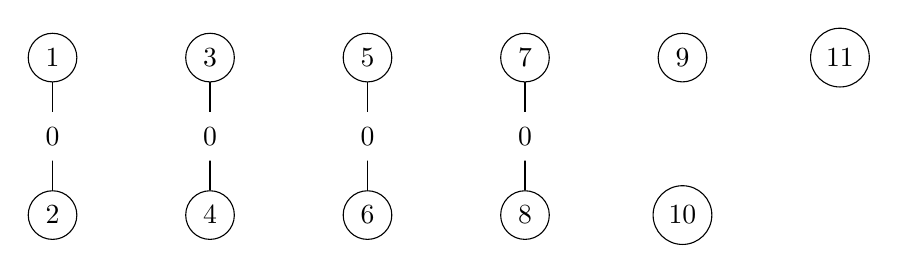
\begin{tikzpicture}

        \begin{scope}[every node/.style={circle,draw}]
          \node (1)  at (0,2)  {1};
          \node (2)  at (0,0)  {2};
          \node (3)  at (2,2)  {3};
          \node (4)  at (2,0)  {4};
          \node (5)  at (4,2)  {5};
          \node (6)  at (4,0)  {6};
          \node (7)  at (6,2)  {7};
          \node (8)  at (6,0)  {8};
          \node (9)  at (8,2)  {9};
          \node (10) at (8,0)  {10};
          \node (11) at (10,2) {11};
        \end{scope}

        \begin{scope}[every node/.style={fill=white,circle}]

          \begin{scope}[every edge/.style={draw}]
            \path (1)  edge node {$0$} (2);
            \path (3)  edge node {$0$} (4);
            \path (5)  edge node {$0$} (6);
            \path (7)  edge node {$0$} (8);
          \end{scope}
        \end{scope}

      \end{tikzpicture}
      \caption{$\rho_0$ est une 4-transposition}
    \end{center}
  \end{figure}

  \paragraph{}
  Maitenant plaçons un carré alterné entre $\rho_0$ et $\rho_4$.

  \begin{figure}[H]
    \begin{center}
      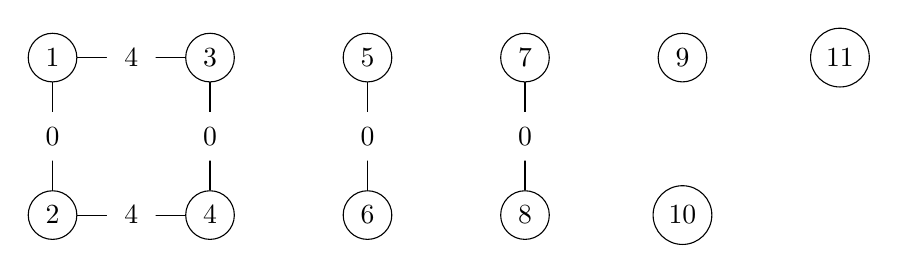
\begin{tikzpicture}

        \begin{scope}[every node/.style={circle,draw}]
          \node (1)  at (0,2)  {1};
          \node (2)  at (0,0)  {2};
          \node (3)  at (2,2)  {3};
          \node (4)  at (2,0)  {4};
          \node (5)  at (4,2)  {5};
          \node (6)  at (4,0)  {6};
          \node (7)  at (6,2)  {7};
          \node (8)  at (6,0)  {8};
          \node (9)  at (8,2)  {9};
          \node (10) at (8,0)  {10};
          \node (11) at (10,2) {11};
        \end{scope}

        \begin{scope}[every node/.style={fill=white,circle}]

          \begin{scope}[every edge/.style={draw}]
            \path (1)  edge node {$0$} (2);
            \path (3)  edge node {$0$} (4);
            \path (5)  edge node {$0$} (6);
            \path (7)  edge node {$0$} (8);
            \path (1)  edge node {$4$} (3);
            \path (2)  edge node {$4$} (4);
          \end{scope}
        \end{scope}

      \end{tikzpicture}
      \caption{Cas 1: carré alterné}
    \end{center}
  \end{figure}

  \paragraph{}
  Par le lemme précédent, on doit trouver une suite de carré alternés jusqu'à ce que la différence ne soit que deux. En partant du carré $[\rho_0,\rho_4]$, cette suite a une taille d'au moins 3 carrés. Il est possible de le faire avec 5 carrés mais il faudrait 12 points ce que nous n'avons pas. Donc la suite est monotone et donc linéaire.

  \paragraph{}
  En partant du carré $[\rho_0,\rho_4]$ on peut aller au carré $[\rho_1,\rho_4]$ ou au carré $[\rho_0,\rho_3]$. Mais si nous n'utilisons pas les involutions $\rho_0$ maintenant, nous ne pourrons jamais les utiliser plus loin car notre suite est linaire et monotone et donc nous ne réutiliserons jamais l'involution $\rho_0$ dans la suite. Les deux arêtes isolées occupent 4 points et la suite de carrés que nous formons va en utiliser 8, donc il faut que nous utilisions au moins une de ces arêtes isolées sinon nous n'aurons pas assez de points. La carré suivant est donc $[\rho_0,\rho_3]$.

  \paragraph{}
  Vu que la suite est linéaire, le carré suivant doit être $[\rho_0, \rho_2]$. La différence des indices de ce carré n'est que de deux, on doit donc relier un arête $\rho_1$ dessus ce qui nous donne le graphe:


  \begin{figure}[H]
    \begin{center}
      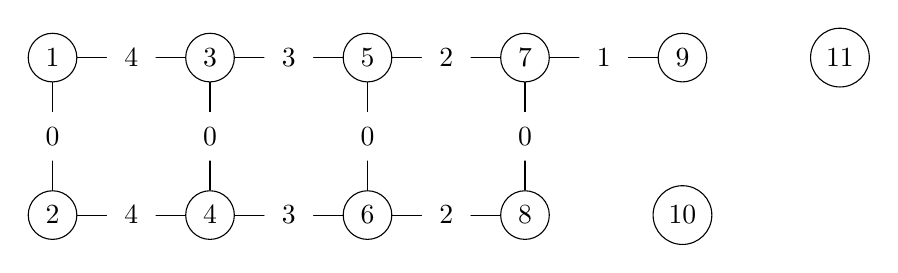
\begin{tikzpicture}

        \begin{scope}[every node/.style={circle,draw}]
          \node (1)  at (0,2)  {1};
          \node (2)  at (0,0)  {2};
          \node (3)  at (2,2)  {3};
          \node (4)  at (2,0)  {4};
          \node (5)  at (4,2)  {5};
          \node (6)  at (4,0)  {6};
          \node (7)  at (6,2)  {7};
          \node (8)  at (6,0)  {8};
          \node (9)  at (8,2)  {9};
          \node (10) at (8,0)  {10};
          \node (11) at (10,2) {11};
        \end{scope}

        \begin{scope}[every node/.style={fill=white,circle}]

          \begin{scope}[every edge/.style={draw}]
            \path (1)  edge node {$0$} (2);
            \path (3)  edge node {$0$} (4);
            \path (5)  edge node {$0$} (6);
            \path (7)  edge node {$0$} (8);
            \path (7)  edge node {$1$} (9);
            \path (5)  edge node {$2$} (7);
            \path (6)  edge node {$2$} (8);
            \path (3)  edge node {$3$} (5);
            \path (4)  edge node {$3$} (6);
            \path (1)  edge node {$4$} (3);
            \path (2)  edge node {$4$} (4);
          \end{scope}
        \end{scope}

      \end{tikzpicture}
      \caption{Cas 1.1: doubles carrés alternés}
    \end{center}
  \end{figure}

  \paragraph{}
  Pour relier les deux derniers points, uniquement 2 arêtes sont nécessaires mais alors le nombre total d'arêtes serait impair ce qui interdit. Il faut donc former un carré alterné ou une arête double. Le carré alterné est impossible car le nombre de points est insuffisant. Il faut donc utiliser une arête double dont la différence des indices est exactement 2 . Toutes les arêtes $\rho_0$ on déjà été utilisées, les seules possibilités sont une arête double $(\rho_1,\rho_3)$ ou une arête double $(\rho_2,\rho_4)$ mais alors soit le nombre d'arêtes $\rho_3$ soit $\rho_4$ devient impair. Donc c'est impossible.
\end{proof}

\begin{lemma}
  Dans un graphe CPR de rang 5 avec 11 points, il est impossible d'avoir une arête double  entre $\rho_0$ et $\rho_4$.\footnote{La preuve de ce théorème est fausse car elle n'envisage pas tous les cas correctement, elle nécessiterait un peu plus d'explications ainsi que quelques précisions à certains endroits}
\end{lemma}

\begin{proof}
  Pour pouvoir étendre cette arête double, il faut utiliser un carré alterné, les possibilités sont soit $[\rho_0, \rho_3]$ soit $[\rho_1, \rho_4]$. Cette deux solutions sont duales donc nous n'étudierons que la première. Il s'agit d'un carré alterné que nous devons à son tour étendre avec $[\rho_0, \rho_2]$ car nous devons rester linéaire. On a donc la graphe suivant:

  \begin{figure}[H]
    \begin{center}
      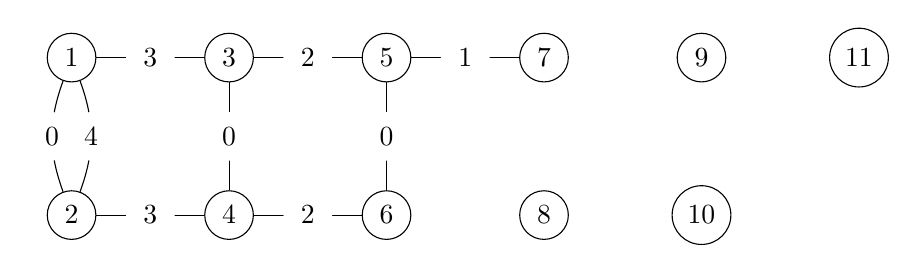
\begin{tikzpicture}

        \begin{scope}[every node/.style={circle,draw}]
          \node (1)  at (0,2)  {1};
          \node (2)  at (0,0)  {2};
          \node (3)  at (2,2)  {3};
          \node (4)  at (2,0)  {4};
          \node (5)  at (4,2)  {5};
          \node (6)  at (4,0)  {6};
          \node (7)  at (6,2)  {7};
          \node (8)  at (6,0)  {8};
          \node (9)  at (8,2)  {9};
          \node (10) at (8,0)  {10};
          \node (11) at (10,2) {11};
        \end{scope}

        \begin{scope}[every node/.style={fill=white,circle}]

          \begin{scope}[every edge/.style={draw}]
            \path (1)  edge[bend right=20] node {$0$} (2);
            \path (3)  edge node {$0$} (4);
            \path (5)  edge node {$0$} (6);
            \path (5)  edge node {$1$} (7);
            \path (3)  edge node {$2$} (5);
            \path (4)  edge node {$2$} (6);
            \path (1)  edge node {$3$} (3);
            \path (2)  edge node {$3$} (4);
            \path (1)  edge[bend left=20] node {$4$} (2);
          \end{scope}
        \end{scope}

      \end{tikzpicture}
      \caption{Cas 1.1.2: doubles carrés alternés et arêtes doublées}
    \end{center}
  \end{figure}

  \paragraph{}
  Nous avons deux problèmes dans ce graphe pour le moment: il n'y a qu'une arête $\rho_4$ et si on relie les points manquants par des arêtes simples, on aura un nombre impaire d'arêtes.\footnote{À partir d'ici c'est incomplet (peut-être faux)}

  \paragraph{}
  Pour pouvoir placer une arête $\rho_4$, nous devons avant placer une arête $\rho_2$ et une arête $\rho_3$. En tout celà utilise 3 points hors des 4 qu'il nous reste. Concernant l'arête double ou le carré alterné, ils ne peuvent être placé sur les points déjà utilisés du graphe actuel. Il faut donc les placer parmi les points non utilisés. Le carré alterné utilise 4 points tandis que l'arête double n'en utilise que deux. Si on place l'arête double à l'extrémité d'une chaîne, elle ne consomme qu'un point. Dans ce cas, il faudrait 3 point pour aller jusque $\rho_4$ et une arête double ensuite. Sauf qu'on ne peut pas placer d'arête double après $\rho_4$, en effet on devrait avoir l'arête double $(\rho_3, \rho_5)$ mais $\rho_5$ n'existe pas.


\end{proof}

\subsection{Main theorems}

\begin{lemma}
  $\rho_0$ (et donc $\rho_4$) ne peut être une 4-transposition.
\end{lemma}

\begin{proof}
  Plaçons la 4-transposition sur le graphe, ajoutons maintenant $\rho_4$ qui doit commuter avec $\rho_0$. Nous pouvons utiliser les motifs suivants:
  \begin{enumerate}
    \item Former un carré alterné
    \item Doubler une arête existante
    \item Relier deux points jusque là fixes
  \end{enumerate}

  \paragraph{}
  La dernière possibilité ne peut être utilisée qu'une seule fois car après nous n'avons plus assez de points fixes. Mais que $\rho_4$ soit une 2-transposition ou une 4-transposition, il reste encore au moins une autre arête à placer. Nous devons dès lors utiliser les deux autres possibilités mais nous avons prouvé qu'elles ne mênent à rien. Donc $\rho_4$ ne peut être une 4-transposition.

\end{proof}

On peut maintenant diviser notre analyse en deux cas en fonction de la disposition des 4-transposition

\begin{enumerate}
  \item $\rho_1$ est une 4-transposition
  \item $\rho_1$ n'est pas une 4-transposition. Si $\rho_3$ est une 4-transposition, il suffit de prendre le dual pour se ramener au premier cas.
\end{enumerate}

\subsubsection{$\rho_1$ est une 4-transposition}

\begin{theorem}
  Si $\rho_1$ est une 4-transposition, alors un générateur peut être écrit comme le produit des autres et donc cet ensemble de "générateurs" n'engendre pas un sggi.
\end{theorem}

\begin{proof}
  Rappelons que par les deux lemmes qui commencent cette section, nous savons que les arêtes $\rho_0$ et $\rho_4$ ne peuvent pas partager de sommet.


  Dessinons donc un graphe sue lequel nous représentons la 4-transposition $\rho_1$, elle doit commuter avec $\rho_3$ et $\rho_4$. Envisageons les différentes possibilité pour $\rho_4$, elle peut soit former un carré alterné, soit doubler deux arêtes, soit doubler une arête et relier deux points encore fixes. Enviageons le premier cas, celui où elle forme un carré alterné avec $\rho_4$.

  \paragraph{}
  Si $\rho_4$ forme un carré alterné avec $\rho_1$, il doit être adjacent à un carré alterné entre $\rho_3$ et $\rho_1$ ($\rho_2$ et $\rho_4$ n'est pas envisageable car $\rho_4$ est une 2-transposition). Ces carrés doivent être reliés au reste du graphe par une arête $\rho_2$, cette arête ne fait partie d'aucun carré alterné donc elle doit forcément relier le carré au l'arête $\rho_1$. On se trouve donc avec le graphe suivant:

  \begin{figure}[H]
    \begin{center}
      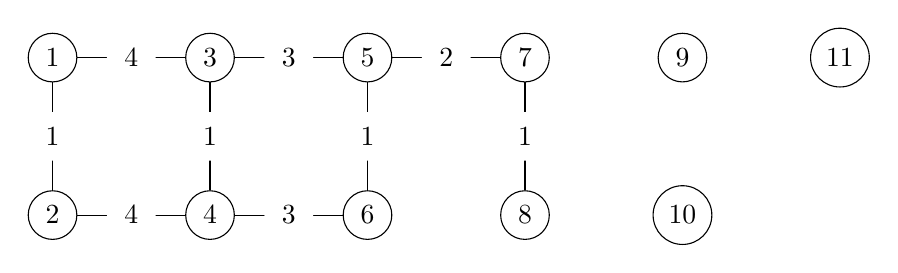
\begin{tikzpicture}

        \begin{scope}[every node/.style={circle,draw}]
          \node (1)  at (0,2)  {1};
          \node (2)  at (0,0)  {2};
          \node (3)  at (2,2)  {3};
          \node (4)  at (2,0)  {4};
          \node (5)  at (4,2)  {5};
          \node (6)  at (4,0)  {6};
          \node (7)  at (6,2)  {7};
          \node (8)  at (6,0)  {8};
          \node (9)  at (8,2)  {9};
          \node (10) at (8,0)  {10};
          \node (11) at (10,2) {11};
        \end{scope}

        \begin{scope}[every node/.style={fill=white,circle}]

          \begin{scope}[every edge/.style={draw}]
            \path (1)  edge node {$1$} (2);
            \path (3)  edge node {$1$} (4);
            \path (5)  edge node {$1$} (6);
            \path (7)  edge node {$1$} (8);
            \path (5)  edge node {$2$} (7);
            \path (3)  edge node {$3$} (5);
            \path (4)  edge node {$3$} (6);
            \path (1)  edge node {$4$} (3);
            \path (2)  edge node {$4$} (4);
          \end{scope}
        \end{scope}

      \end{tikzpicture}
      \caption{Un carré alterné et son voisin engendré}
    \end{center}
  \end{figure}

  \paragraph{}
  Maintenant si nous essayons de placer les arêtes $\rho_0$, nous avons un problème car nous n'avons qu'une extrémité d'arête $\rho_1$ disponible pour les relier au reste. Il faut donc former un carré alterné entre $\rho_0$ et $\rho_2$ et relier ce carré au reste grâce à l'arête $\rho_1$. On a le graphe suivant.
  % TODO une petite preuve ?

  \begin{figure}[H]
    \begin{center}
      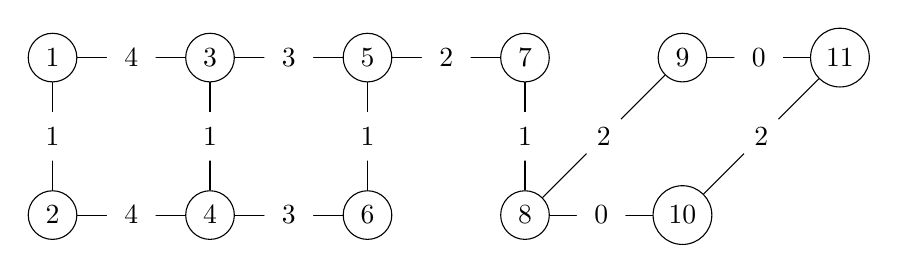
\begin{tikzpicture}

        \begin{scope}[every node/.style={circle,draw}]
          \node (1)  at (0,2)  {1};
          \node (2)  at (0,0)  {2};
          \node (3)  at (2,2)  {3};
          \node (4)  at (2,0)  {4};
          \node (5)  at (4,2)  {5};
          \node (6)  at (4,0)  {6};
          \node (7)  at (6,2)  {7};
          \node (8)  at (6,0)  {8};
          \node (9)  at (8,2)  {9};
          \node (10) at (8,0)  {10};
          \node (11) at (10,2) {11};
        \end{scope}

        \begin{scope}[every node/.style={fill=white,circle}]

          \begin{scope}[every edge/.style={draw}]
            \path (9)  edge node {$0$} (11);
            \path (8)  edge node {$0$} (10);
            \path (1)  edge node {$1$} (2);
            \path (3)  edge node {$1$} (4);
            \path (5)  edge node {$1$} (6);
            \path (7)  edge node {$1$} (8);
            \path (5)  edge node {$2$} (7);
            \path (8)  edge node {$2$} (9);
            \path (10) edge node {$2$} (11);
            \path (3)  edge node {$3$} (5);
            \path (4)  edge node {$3$} (6);
            \path (1)  edge node {$4$} (3);
            \path (2)  edge node {$4$} (4);
          \end{scope}
        \end{scope}

      \end{tikzpicture}
      \caption{Un carré alterné et son voisin engendré}
    \end{center}
  \end{figure}

  \paragraph{}
  Pour restaurer la parité, il faut encore utiliser une arête $\rho_2$. Il n'y a que deux possibilités pour une telle arête: il faut doubler une des arêtes $\rho_4$.

  \paragraph{}
  Maitenant soit nous nous arétons là et alors $\rho_3$ est une 2-transposition, soit nous continuons à rajouter deux arêtes $\rho_3$.

  \paragraph{}
  Analysons les possibilités pour ces dernières, seulement deux possibilités sont disponibles, entre les point $1$ et $2$ ou entre les points $10$ et $11$.

  \paragraph{}
  Ceci conclut notre analyse pour le carré alterné en $\rho_1$ et $\rho_4$, envisageons maitenant la seconde possibilité, celle d'une arête double entre $\rho_0$ et $\rho_4$. Nous devons placer un carré alterné à coté vu que nous voulons le relier au reste. On a donc le graphe suivant

  \begin{figure}[H]
    \begin{center}
      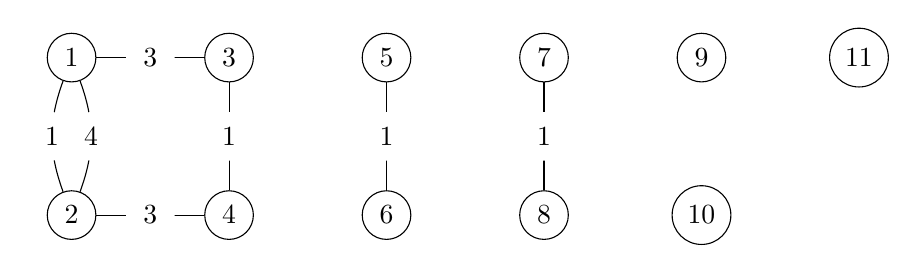
\begin{tikzpicture}

        \begin{scope}[every node/.style={circle,draw}]
          \node (1)  at (0,2)  {1};
          \node (2)  at (0,0)  {2};
          \node (3)  at (2,2)  {3};
          \node (4)  at (2,0)  {4};
          \node (5)  at (4,2)  {5};
          \node (6)  at (4,0)  {6};
          \node (7)  at (6,2)  {7};
          \node (8)  at (6,0)  {8};
          \node (9)  at (8,2)  {9};
          \node (10) at (8,0)  {10};
          \node (11) at (10,2) {11};
        \end{scope}

        \begin{scope}[every node/.style={fill=white,circle}]

          \begin{scope}[every edge/.style={draw}]
            \path (1)  edge[bend right=20] node {$1$} (2);
            \path (3)  edge node {$1$} (4);
            \path (5)  edge node {$1$} (6);
            \path (7)  edge node {$1$} (8);
            \path (1)  edge node {$3$} (3);
            \path (2)  edge node {$3$} (4);
            \path (1)  edge[bend left=20] node {$4$} (2);
          \end{scope}
        \end{scope}

      \end{tikzpicture}
      \caption{Un carré alterné et son voisin engendré}
    \end{center}
  \end{figure}


\end{proof}

\begin{theorem}
  Soit un sggi de rang 5 sur $A_{11}$. Alors ce sggi contient exactement une 4-transposition.
\end{theorem}

Il nous reste deux cas à analyser, celui où il y a deux 4-transpositions, celles-ci sont alors forcément en $\rho_1$ et $\rho_2$ (à la dualité près) et celui où on a trois 4-transpositions qui sont alors positionnées en $\rho_1$, $\rho_2$ et $\rho_3$.

\begin{proof}
  En partant du graphe de la preuve précédente, si on rajoute l'involution $\rho_3$, on l'étend à $A_{11}$.
  En effet, partons du graphe et essayons de rajouter la 2-transposition $\rho_3$, celle-ci doit commuter avec $\rho_0$ et $\rho_1$.
  \begin{figure}[H]
    \begin{center}
      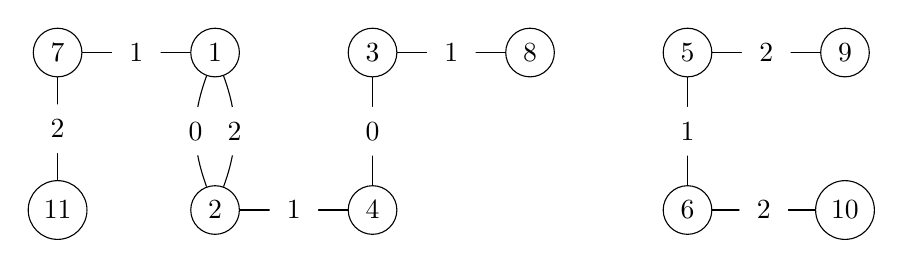
\begin{tikzpicture}

        \begin{scope}[every node/.style={circle,draw}]
          \node (1)  at (0,2)  {1};
          \node (2)  at (0,0)  {2};
          \node (3)  at (2,2)  {3};
          \node (4)  at (2,0)  {4};
          \node (5)  at (6,2)  {5};
          \node (6)  at (6,0)  {6};
          \node (7)  at (-2,2) {7};
          \node (8)  at (4,2)  {8};
          \node (9)  at (8,2)  {9};
          \node (10) at (8,0) {10};
          \node (11) at (-2,0) {11};
        \end{scope}

        \begin{scope}[every node/.style={fill=white,circle}]

          \begin{scope}[every edge/.style={draw}]
            \path (1)  edge[bend right=20] node {$0$} (2);
            \path (3)  edge node {$0$} (4);
            \path (1)  edge node {$1$} (7);
            \path (2)  edge node {$1$} (4);
            \path (3)  edge node {$1$} (8);
            \path (5)  edge node {$1$} (6);
            \path (1)  edge[bend left=20] node {$2$} (2);
            \path (5)  edge node {$2$} (9);
            \path (6)  edge node {$2$} (10);
            \path (7)  edge node {$2$} (11);
          \end{scope}
        \end{scope}

      \end{tikzpicture}
      \caption{Example of subgroup of sggi of type 2}
    \end{center}
  \end{figure}

  \paragraph{}
  Nous devons utiliser 2 arêtes $\rho_3$, pour cela nous avons trois possibilités, sachant que nous pouvons ignorer les arêtes $\rho_2$.
  \begin{enumerate}
    \item Relier deux points non reliés
    \item Doubler une arête
    \item Former un carré alterné
  \end{enumerate}

  \paragraph{}
  Dans la composante de gauche, suite à l'alternance des arêtes $\rho_0$ et $\rho_1$ il n'est pas possible de former un carré alterné ou une arête double, la seule possibilité est une arête qui partirait du point 11. Dans la composante de droite, les possibilités sont plus variés. On doit placer deux arêtes en tout et pour le moment nous n'avons trouvé qu'un point d'attache potentiel. Il en faut donc au moins 3 autres parmi les 4 points qui compose cette composante. Nous sommes donc obligé d'utiliser le point 5 ou le point 6 mais dans ce cas, nous sommes obligés de doubler l'arête $\rho_1$ présente à cet endroit. Pour la dernière arête soit nous relions les deux points restants dans la composante de droite soit nous relions un de ces points à l'autre composante.

  \paragraph{}
  Dans le premier cas nous ne pourrons jamais atteindre $A_{11}$. En effet, nous avons le graphe suivant
  \begin{figure}[H]
    \begin{center}
      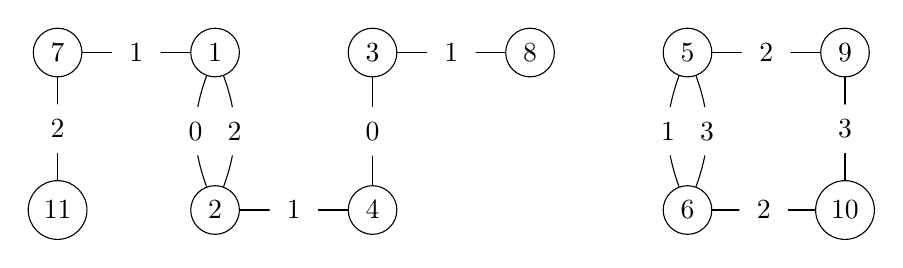
\begin{tikzpicture}

        \begin{scope}[every node/.style={circle,draw}]
          \node (1)  at (0,2)  {1};
          \node (2)  at (0,0)  {2};
          \node (3)  at (2,2)  {3};
          \node (4)  at (2,0)  {4};
          \node (5)  at (6,2)  {5};
          \node (6)  at (6,0)  {6};
          \node (7)  at (-2,2) {7};
          \node (8)  at (4,2)  {8};
          \node (9)  at (8,2)  {9};
          \node (10) at (8,0) {10};
          \node (11) at (-2,0) {11};
        \end{scope}

        \begin{scope}[every node/.style={fill=white,circle}]

          \begin{scope}[every edge/.style={draw}]
            \path (1)  edge[bend right=20] node {$0$} (2);
            \path (3)  edge node {$0$} (4);
            \path (1)  edge node {$1$} (7);
            \path (2)  edge node {$1$} (4);
            \path (3)  edge node {$1$} (8);
            \path (5)  edge[bend right=20] node {$1$} (6);
            \path (1)  edge[bend left=20] node {$2$} (2);
            \path (5)  edge node {$2$} (9);
            \path (6)  edge node {$2$} (10);
            \path (7)  edge node {$2$} (11);
            \path (5)  edge[bend left=20] node {$3$} (6);
            \path (9)  edge node {$3$} (10);
          \end{scope}
        \end{scope}

      \end{tikzpicture}
      \caption{Example of subgroup of sggi of type 2}
    \end{center}
  \end{figure}

  \paragraph{}
  Dans cet graphe, $\rho_2$ et $\rho_3$ commute donc ce graphe ne peut être celui d'un groupe semi-simple. Même si nous rajoutons des involutions, cela ne changera rien à ce résultat et le graphe ne pourra jamais être celui d'$A_{11}$. La seule possibilité qu'il nous reste est le premier graphe.

  \begin{figure}[H]
    \begin{center}
      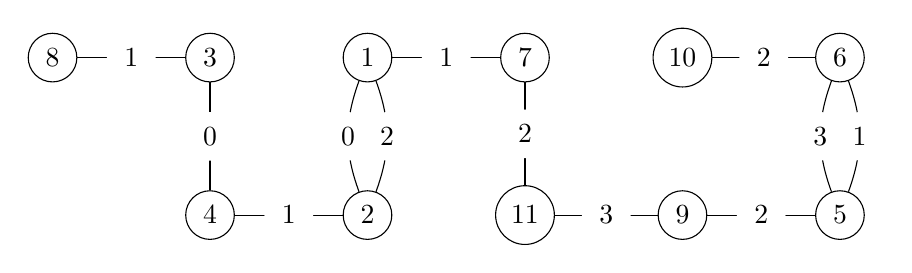
\begin{tikzpicture}

        \begin{scope}[every node/.style={circle,draw}]
          \node (1)  at (2,2)  {1};
          \node (2)  at (2,0)  {2};
          \node (3)  at (0,2)  {3};
          \node (4)  at (0,0)  {4};
          \node (5)  at (8,0)  {5};
          \node (6)  at (8,2)  {6};
          \node (7)  at (4,2)  {7};
          \node (8)  at (-2,2) {8};
          \node (9)  at (6,0)  {9};
          \node (10) at (6,2) {10};
          \node (11) at (4,0) {11};
        \end{scope}

        \begin{scope}[every node/.style={fill=white,circle}]

          \begin{scope}[every edge/.style={draw}]
            \path (1)  edge[bend right=20] node {$0$} (2);
            \path (3)  edge node {$0$} (4);
            \path (1)  edge node {$1$} (7);
            \path (2)  edge node {$1$} (4);
            \path (3)  edge node {$1$} (8);
            \path (5)  edge[bend right=20] node {$1$} (6);
            \path (1)  edge[bend left=20] node {$2$} (2);
            \path (5)  edge node {$2$} (9);
            \path (6)  edge node {$2$} (10);
            \path (7)  edge node {$2$} (11);
            \path (5)  edge[bend left=20] node {$3$} (6);
            \path (9)  edge node {$3$} (11);
          \end{scope}
        \end{scope}

      \end{tikzpicture}
      \caption{Example of subgroup of sggi of type 2}
    \end{center}
  \end{figure}

\end{proof}

\begin{lemma}
  Ce graphe engendre $A_{11}$.
\end{lemma}

\subsubsection{$\rho_1$ n'est pas une 4-transposition}

\paragraph{}
Par le lemme précédent, il faut au moins une 4-transposition. Celle-ci doit forcément se trouver en $\rho_2$.

\paragraph{}
Dans ce cas, aucun générateur n'est redondante. En effet si on supprimait un générateur, on aurait un sggi de rang 4 avec une seule 4-transposition mais nous avons prouvé que, dans ce cas, il ne peut engendrer $A_11$.

\paragraph{}
Commençons par trouver tous les sggis de rang 5 qui sont valables.

\begin{theorem}
  Les seuls graphes CPR de rang 5 sur 11 points sont les suivants:

\end{theorem}

\paragraph{}
Nous devons prouver qu'il n'y a aucun C-group de rang 5 qui engendre $A_{11}$.

\begin{theorem}
  Soit un sggi de rang 5 sur $A_{11}$. Alors ce sggi n'est pas un C-group.
\end{theorem}

\begin{proof}
  Nous allons construire toutes les possibilités de graphe CPR. Partons d'un graphe avec juste la 4-transposition $\rho_2$.

  \begin{figure}[H]
    \begin{center}
      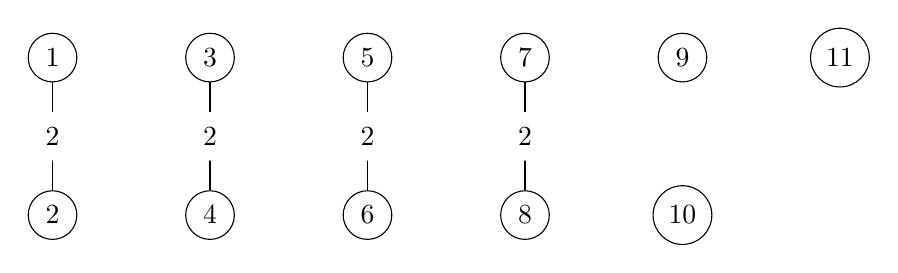
\begin{tikzpicture}

        \begin{scope}[every node/.style={circle,draw}]
          \node (1)  at (0,2)  {1};
          \node (2)  at (0,0)  {2};
          \node (3)  at (2,2)  {3};
          \node (4)  at (2,0)  {4};
          \node (5)  at (4,2)  {5};
          \node (6)  at (4,0)  {6};
          \node (7)  at (6,2)  {7};
          \node (8)  at (6,0)  {8};
          \node (9)  at (8,2)  {9};
          \node (10) at (8,0)  {10};
          \node (11) at (10,2) {11};
        \end{scope}

        \begin{scope}[every node/.style={fill=white,circle}]

          \begin{scope}[every edge/.style={draw}]
            \path (1)  edge node {$2$} (2);
            \path (3)  edge node {$2$} (4);
            \path (5)  edge node {$2$} (6);
            \path (7)  edge node {$2$} (8);
          \end{scope}
        \end{scope}

      \end{tikzpicture}
      \caption{[1, 5, 1010, 232, 381]}
    \end{center}
  \end{figure}

\paragraph{}
Nous allons essayer d'ajouter les involutions $\rho_0$ et $\rho_4$. Celles-ci doivent commuter avec $\rho_2$. Pour chaque involution nous devons choisir entre les 3 possibilités suivantes:
\begin{enumerate}
  \item Faire un arête double avec $\rho_2$ et reliés deux points qui sont, pour le moment, fixes.
  \item Faire deux arêtes doubles avec $\rho_2$.
  \item Faire un carré alterné avec $\rho_2$.
\end{enumerate}

\paragraph{}
S'il n'y a qu'une seule 4-transposition, alors nous avons 12 arêtes pour relier 11 points soit 2 de plus que le strict minimum. Dès lors, lorsque nous ajoutons une arête, elle doit toujours relier deux composantes différentes, sauf à deux occasions. Quand nous formons un carré alterné, nous utilisons une de ces deux arêtes et il se passe la même chose quand nous formons une arête double.

\paragraph{}
Parmi les trois possibilités, la seconde est impossible car si nous l'appliquons, nous aurons déjà utilisé nous deux arêtes "joker". Quand nous allons vouloir ajouter la seconde involution, nous n'en aurons plus mais toutes les possibilités en demande au moins une.

\paragraph{}
Remarquons qu'il est impossible de faire le même choix pour $\rho_0$ et $\rho_4$. Si nous utilisions deux fois la première proposition, il nous faudrait 4 points fixes mais nous n'en avons que 3. Si nous choisissons la troisième proposition, nous ne pouvons pas superposer les carrés sans former deux arêtes doubles, ce qui est impossible.

\paragraph{}
Les deux carrés ne peuvent pas être adjacents non plus car on aurait des arêtes $\rho_0$ et $\rho_4$ adjacentes mais nous ne pourions plus former de carré alterné pour créer un motif valable.

\paragraph{}
Dans le cas deux deux carrés disjoints, nous ne pouvons pas les relier car nous avons utilisé toutes les arêtes des involutions $\rho_0$, $\rho_2$ et $\rho_4$. Il ne nous reste donc que des arêtes des involutions $\rho_1$ et $\rho_3$ et celles-ce ne peuvent partager un sommet sans former un carré alterné ou une arêted double mais ça c'est impossible.

\paragraph{}
La seule possibilité qu'il nous reste est de choisir que $\rho_0$ reliera deux point fixes et doublera une arête et que $\rho_4$ formera un carré alterné (l'autre cas est le dual). On a donc le graphe suivant:


\begin{figure}[H]
  \begin{center}
    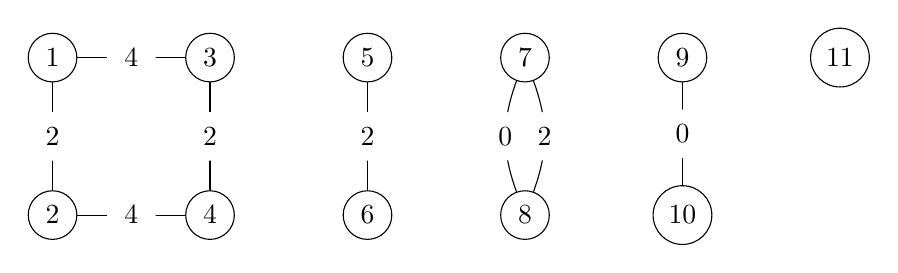
\begin{tikzpicture}

      \begin{scope}[every node/.style={circle,draw}]
        \node (1)  at (0,2)  {1};
        \node (2)  at (0,0)  {2};
        \node (3)  at (2,2)  {3};
        \node (4)  at (2,0)  {4};
        \node (5)  at (4,2)  {5};
        \node (6)  at (4,0)  {6};
        \node (7)  at (6,2)  {7};
        \node (8)  at (6,0)  {8};
        \node (9)  at (8,2)  {9};
        \node (10) at (8,0)  {10};
        \node (11) at (10,2) {11};
      \end{scope}

      \begin{scope}[every node/.style={fill=white,circle}]

        \begin{scope}[every edge/.style={draw}]
          \path (9)  edge node {$0$} (10);
          \path (7)  edge[bend right=20] node {$0$} (8);
          \path (1)  edge node {$2$} (2);
          \path (3)  edge node {$2$} (4);
          \path (5)  edge node {$2$} (6);
          \path (7)  edge[bend left=20] node {$2$} (8);
          \path (1)  edge node {$4$} (3);
          \path (2)  edge node {$4$} (4);
        \end{scope}
      \end{scope}

    \end{tikzpicture}
    \caption{[1, 5, 1010, 232, 381]}
  \end{center}
\end{figure}

\paragraph{}
À partir de maintenant, si nous rajoutons une arête, elle doit relier deux composantes connexes distinctes du graphe.

\paragraph{}
Le carré alterné doit être relié par une arête $\rho_3$. Cette arête peut aller sur le point fixe ou sur l'arête isolée $\rho_2$. Néanmoins du point fixe, il est impossible de continuer car il nous faut une arête $\rho_2$ ou $\rho_4$ mais elles ont toutes déjà été placées. Donc il y a une arête $\rho_3$ entre le carré alterné et l'arête isolée $\rho_2$.

\paragraph{}
Vu que nous n'avons qu'une arête $\rho_2$ isolée, nous n'avons qu'un moyen de relier les arêtes $\rho_1$ au carré. Toutes ces arêtes doivent donc être dans la même partie du graphe.

\paragraph{}
Remarquons que l'arête double $(\rho_0, \rho_2)$ ainsi que l'arête simple $\rho_0$ ne peuvent être relié que par des arête $\rho_1$. Vu que nous n'avons que deux arêtes $\rho_1$ et que toutes ces arêtes sont situés dans la même branche du graphe, une de ces arêtes doit être à l'extémité de la branche et doit être relié à l'autre avec une arête $\rho_1$. On stade actuel, nous avons le graphe suivant:

\begin{figure}[H]
  \begin{center}
    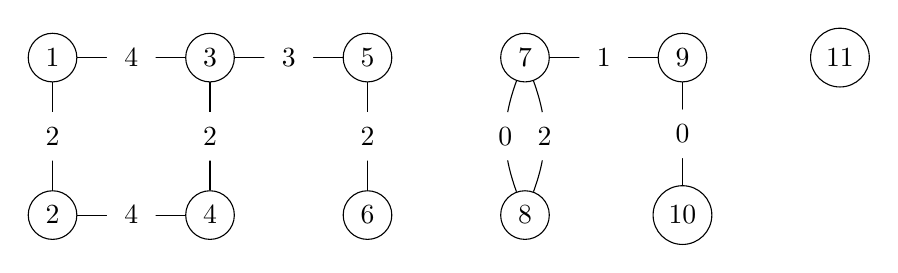
\begin{tikzpicture}

      \begin{scope}[every node/.style={circle,draw}]
        \node (1)  at (0,2)  {1};
        \node (2)  at (0,0)  {2};
        \node (3)  at (2,2)  {3};
        \node (4)  at (2,0)  {4};
        \node (5)  at (4,2)  {5};
        \node (6)  at (4,0)  {6};
        \node (7)  at (6,2)  {7};
        \node (8)  at (6,0)  {8};
        \node (9)  at (8,2)  {9};
        \node (10) at (8,0)  {10};
        \node (11) at (10,2) {11};
      \end{scope}

      \begin{scope}[every node/.style={fill=white,circle}]

        \begin{scope}[every edge/.style={draw}]
          \path (9)  edge node {$0$} (10);
          \path (7)  edge[bend right=20] node {$0$} (8);
          \path (7)  edge node {$1$} (9);
          \path (1)  edge node {$2$} (2);
          \path (3)  edge node {$2$} (4);
          \path (5)  edge node {$2$} (6);
          \path (7)  edge[bend left=20] node {$2$} (8);
          \path (3)  edge node {$3$} (5);
          \path (1)  edge node {$4$} (3);
          \path (2)  edge node {$4$} (4);
        \end{scope}
      \end{scope}

    \end{tikzpicture}
    \caption{[1, 5, 1010, 232, 381]}
  \end{center}
\end{figure}

\paragraph{}
À ce stade, il reste une arête $\rho_1$ et une arête $\rho_3$ à placer. L'arête $\rho_1$ permet de relier le l'arête simple $\rho_2$ à la grande composante. On a deux façons de le faire en fonction du sens dans lequel on attache cette dernière. L'arête $\rho_3$ quant à elle doit servir à relier le point fixe au reste. Le seul point d'attche pour cette arête $\rho_3$ est le carré alterné. On a trois possibilités, on fonction si les arêtes $\rho_3$ sont connectées à des sommets opposés sur le carré, si elles sont séparées par une arête $\rho_2$ ou une arête $\rho_4$.

\paragraph{}
En tout, on a donc exactement 6 graphe CPR admissibles pour cette configuration.

\end{proof}

Dans la suite, nous reprendrons la numérotation des sommets décrite à la section~\ref{monodromy-5} (p. \pageref{monodromy-5})

\begin{theorem}
  Aucun des groupes engendré par ces graphes n'est un C-group.
\end{theorem}

\begin{proof}
  D'après la definition d'un C-group, il suffit de trouver deux sous-ensembles de générateurs $S_1$ et $S_2$ tel que $\Gamma_{S_1} \cap \Gamma_{S_2} \neq \Gamma_{S_1 \cap S_2}$.

  \paragraph{}
  Dans notre cas, nous prendrons $S_1 = \{\rho_1, \rho_2\}$, et $S_2 = \{\rho_2, \rho_3, \rho_4\}$. Dans ce cas, $S_1 \cap S_2 = \{\rho_2\}$  et donc $\Gamma_{\rho_2} = \langle (1\ 2)(5\ 6)(7\ 8)(9\ 10) \rangle$. Ce groupe ne contient que deux éléments, l'identité et $\rho_2$. En effet $\rho_2$ est une involution et donc $\rho_2\rho_2 = 1$.

  \paragraph{}
  Étudions plus en détail $S_1$, si nous ne conservons que ces générateurs, le choix que nous avons effectuer concernant la position des arêtes $\rho_3$ le long du carré alterné n'a aucune importance. Nous avons juste deux graphes différents à étudier:

  \begin{figure}[H]
    \begin{center}
      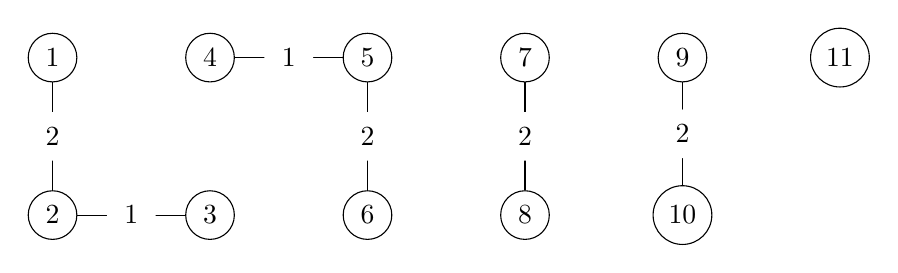
\begin{tikzpicture}

        \begin{scope}[every node/.style={circle,draw}]
          \node (1)  at (0,2)  {1};
          \node (2)  at (0,0)  {2};
          \node (3)  at (2,0)  {3};
          \node (4)  at (2,2)  {4};
          \node (5)  at (4,2)  {5};
          \node (6)  at (4,0)  {6};
          \node (7)  at (6,2)  {7};
          \node (8)  at (6,0)  {8};
          \node (9)  at (8,2)  {9};
          \node (10) at (8,0)  {10};
          \node (11) at (10,2) {11};
        \end{scope}

        \begin{scope}[every node/.style={fill=white,circle}]

          \begin{scope}[every edge/.style={draw}]
            \path (2)  edge node {$1$} (3);
            \path (4)  edge node {$1$} (5);
            \path (1)  edge node {$2$} (2);
            \path (5)  edge node {$2$} (6);
            \path (7)  edge node {$2$} (8);
            \path (9)  edge node {$2$} (10);
          \end{scope}
        \end{scope}

      \end{tikzpicture}
      \caption{[1, 5, 994, 219, 381]}
    \end{center}
  \end{figure}

  \begin{figure}[H]
    \begin{center}
      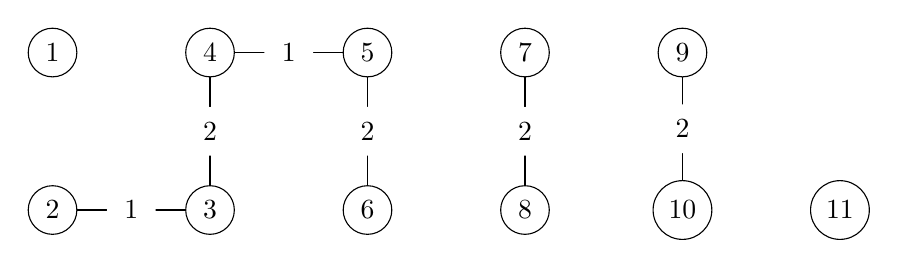
\begin{tikzpicture}

        \begin{scope}[every node/.style={circle,draw}]
          \node (1)  at (0,2)  {1};
          \node (2)  at (0,0)  {2};
          \node (3)  at (2,0)  {3};
          \node (4)  at (2,2)  {4};
          \node (5)  at (4,2)  {5};
          \node (6)  at (4,0)  {6};
          \node (7)  at (6,2)  {7};
          \node (8)  at (6,0)  {8};
          \node (9)  at (8,2)  {9};
          \node (10) at (8,0)  {10};
          \node (11) at (10,0) {11};
        \end{scope}

        \begin{scope}[every node/.style={fill=white,circle}]

          \begin{scope}[every edge/.style={draw}]
            \path (2)  edge node {$1$} (3);
            \path (4)  edge node {$1$} (5);
            \path (3)  edge node {$2$} (4);
            \path (5)  edge node {$2$} (6);
            \path (7)  edge node {$2$} (8);
            \path (9)  edge node {$2$} (10);
          \end{scope}
        \end{scope}

      \end{tikzpicture}
      \caption{[1, 5, 1010, 232, 381]}
    \end{center}
  \end{figure}

  \paragraph{}
  Dans le premier cas, étudions la permutation $(\rho_1\rho_2)^2\rho_1$, elle laisse les points des deux arêtes isolées tel quel car la permutation utilise $\rho_2$ un nombre pair de fois. Les points 3 et 4 restent aussi fixes, mais les points 1 et 2 ainsi que 5 et 6 sont intervertis. On a $(\rho_1\rho_2)^2\rho_1 = (1\ 2)(5\ 6)$, donc $(1\ 2)(5\ 6) \in \Gamma_{S_1}$.

  \paragraph{}
  Dans le second graphe, c'est $(\rho_1\rho_2)^4\rho_1$ qui nous donne le même résultat.

  % TODO Renuméroter les graphes !!!

  \paragraph{}
  Étudions maitenant $S_2$, Dans ce cas, il n'y a que la façon donc nous avons disposé les arêtes $\rho_3$ sur le carré atlerné qui intervient. Ceci nous donne donc trois possibilités.

  \begin{figure}[H]
    \begin{center}
      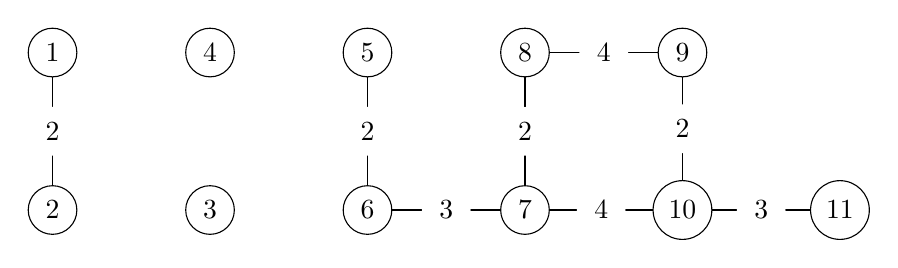
\begin{tikzpicture}

        \begin{scope}[every node/.style={circle,draw}]
          \node (1)  at (0,2)  {1};
          \node (2)  at (0,0)  {2};
          \node (3)  at (2,0)  {3};
          \node (4)  at (2,2)  {4};
          \node (5)  at (4,2)  {5};
          \node (6)  at (4,0)  {6};
          \node (7)  at (6,0)  {7};
          \node (8)  at (6,2)  {8};
          \node (9)  at (8,2)  {9};
          \node (10) at (8,0)  {10};
          \node (11) at (10,0) {11};
        \end{scope}

        \begin{scope}[every node/.style={fill=white,circle}]

          \begin{scope}[every edge/.style={draw}]
            \path (1)  edge node {$2$} (2);
            \path (5)  edge node {$2$} (6);
            \path (7)  edge node {$2$} (8);
            \path (9)  edge node {$2$} (10);
            \path (6)  edge node {$3$} (7);
            \path (10) edge node {$3$} (11);
            \path (7)  edge node {$4$} (10);
            \path (8)  edge node {$4$} (9);
          \end{scope}
        \end{scope}

      \end{tikzpicture}
      \caption{[1, 5, 994, 219, 267]}
    \end{center}
  \end{figure}

  \begin{figure}[H]
    \begin{center}
      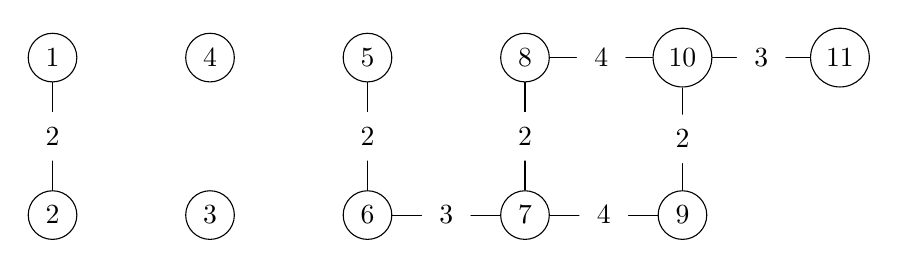
\begin{tikzpicture}

        \begin{scope}[every node/.style={circle,draw}]
          \node (1)  at (0,2)  {1};
          \node (2)  at (0,0)  {2};
          \node (3)  at (2,0)  {3};
          \node (4)  at (2,2)  {4};
          \node (5)  at (4,2)  {5};
          \node (6)  at (4,0)  {6};
          \node (7)  at (6,0)  {7};
          \node (8)  at (6,2)  {8};
          \node (9)  at (8,0)  {9};
          \node (10) at (8,2)  {10};
          \node (11) at (10,2) {11};
        \end{scope}

        \begin{scope}[every node/.style={fill=white,circle}]

          \begin{scope}[every edge/.style={draw}]
            \path (1)  edge node {$2$} (2);
            \path (5)  edge node {$2$} (6);
            \path (7)  edge node {$2$} (8);
            \path (9)  edge node {$2$} (10);
            \path (6)  edge node {$3$} (7);
            \path (10) edge node {$3$} (11);
            \path (7)  edge node {$4$} (9);
            \path (8)  edge node {$4$} (10);
          \end{scope}
        \end{scope}

      \end{tikzpicture}
      \caption{[1, 5, 994, 219, 381]}
    \end{center}
  \end{figure}

  \begin{figure}[H]
    \begin{center}
      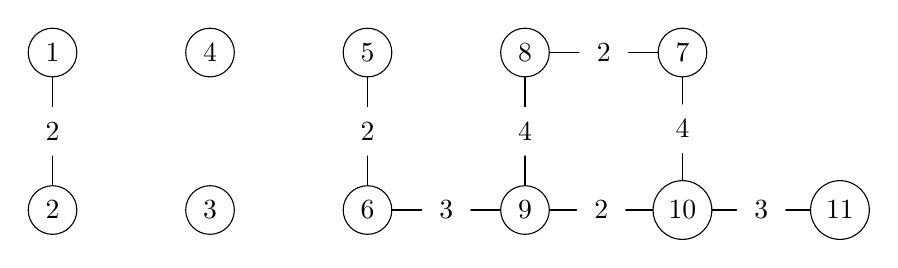
\begin{tikzpicture}

        \begin{scope}[every node/.style={circle,draw}]
          \node (1)  at (0,2)  {1};
          \node (2)  at (0,0)  {2};
          \node (3)  at (2,0)  {3};
          \node (4)  at (2,2)  {4};
          \node (5)  at (4,2)  {5};
          \node (6)  at (4,0)  {6};
          \node (7)  at (8,2)  {7};
          \node (8)  at (6,2)  {8};
          \node (9)  at (6,0)  {9};
          \node (10) at (8,0)  {10};
          \node (11) at (10,0) {11};
        \end{scope}

        \begin{scope}[every node/.style={fill=white,circle}]

          \begin{scope}[every edge/.style={draw}]
            \path (1)  edge node {$2$} (2);
            \path (5)  edge node {$2$} (6);
            \path (7)  edge node {$2$} (8);
            \path (9)  edge node {$2$} (10);
            \path (6)  edge node {$3$} (9);
            \path (10) edge node {$3$} (11);
            \path (7)  edge node {$4$} (10);
            \path (8)  edge node {$4$} (9);
          \end{scope}
        \end{scope}

      \end{tikzpicture}
      \caption{[1, 5, 994, 232, 267]}
    \end{center}
  \end{figure}

\end{proof}

\paragraph{}
Grâce à ces deux théorèmes, on sait qu'il existe une 2-transposition $g$ dont $\rho_2$ est une extension qui est telle que $ g \in \Gamma_{0,1} = S_7$ et $g \in \Gamma_(0,3,4)$ donc $g \in \Gamma_{0,1} \cap \Gamma_(0,3,4)$ mais $g \notin \Gamma_{0,1,3,4} = <\rho_2>$. Donc $\Gamma_{0,1} \cap \Gamma_{0,3,4} \neq \Gamma_{0,1,3,4}$ donc $\Gamma$ ne satisafait pas la propriété d'intersection et n'est donc pas un C-group. Ce qui conclut la preuve du théorème
